\section{Experiments}

\subsection{Training configuration}

\subsection{Comparison to baselines}

\begin{figure}[t]
	\begin{center}
		% \fbox{\rule{0pt}{2in}\rule{0.9\linewidth}{0pt}}
		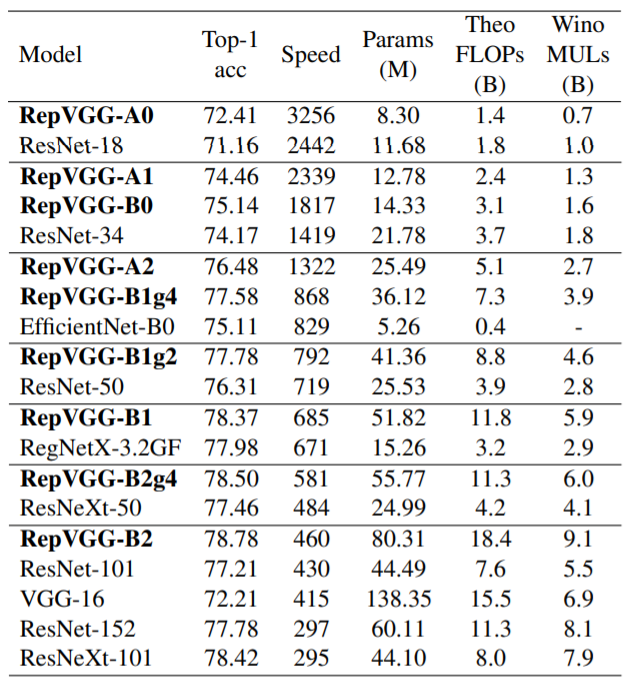
\includegraphics[width=0.8\linewidth]{images/results1.PNG}
	\end{center}
	\caption{RepVGG performance on ImageNet after being trained 120 epochs with simple data augmentation. The speed is measured in examples/second.}
	\label{fig:results1}
\end{figure}

When analyzing the empirical results (see \autoref{fig:results1}) one recognizes the following achievements. 

First the light- and middleweight models of RepVGG-A slightly outperform their ResNet baselines in accuracy, but achieve far higher inference speed. For instance RepVGG-A2 having a comparable amount of parameters to ResNet-50 is only 0.17\% better in accuracy, but therefor 83\% faster. Using interleaved groupwise convolutional layers such increases in speed can further be pushed, e.g. when looking at RepVGG-B1g2 and its counterpart baseline ResNet-152. Achieving the same accuracy RepVGG-B1g2 is a whole 2.66 times faster. 

When looking at the parameter efficiency RepVGG manages to outperfom the historical ResNet and VGG competitors. While achieving the same accuracy RepVGG-B1g2 only needs 69\% of the parameters of ResNet-152. The difference is even higher when comparing RepVGG-A0 to VGG-16 which state a reduction around 94\% of the parameters needed (8.30M compared to 138.35M). Obviously such parameter efficiency gains change when comparing RepVGG to more modern architectures like EfficientNet (14.33M RevVGG-B0 vs. 5.26M EfficientNet-B0) or RegNet (15.26M RegNetX-32.GF vs 41.36M RepVGG-B1g2). As the goal of RepVGG is to gain a good accuracy-speed trade-off while using a plain architecture for inference, such parameter inefficiency are justifiable and difficult to avoid. 

Also it is worth noticing that RepVGG models can of course - at the costs of the amount of parameters needed - keep up with state-of-the-art models. The authors therefore try to make a point by comparing e.g. EfficientNet-B0 to RepVGG-A2 being 1.37\% more accurate and 59\% faster. The question remains whether this can be seen as a valid argument as EfficientNet-B0 uses far less parameters compared to Rep-VGG-A2. If one compares models with approximately equal number of parameters like ResNeXt-50 to RepVGG-A2 such accuracy guarantees will no longer outperform the state-of-the-art models (77.46 vs. 76.48). Nevertheless the speed-up factors remain the strong accomplishment of all RepVGG models (484 ResNeXt-50 vs. 1322 RepVGG-A2). The comparison of ResNeXt-50 and RepVGG-A2 is in addition a perfect proof of the thesis that speed cannot be approximated with FLOPs. If so ResNeXt-50 should have been faster in inference as having less theoretical FLOPs compared to RepVGG-A2 (4.2 vs. 5.1). Winograd multiplications on the other hand seem to work as a better metric to derive speed comparisons (4.1 ResNeXt-50 vs. 2.7 RepVGG-A2). 

\begin{figure}[t]
	\begin{center}
		% \fbox{\rule{0pt}{2in}\rule{0.9\linewidth}{0pt}}
		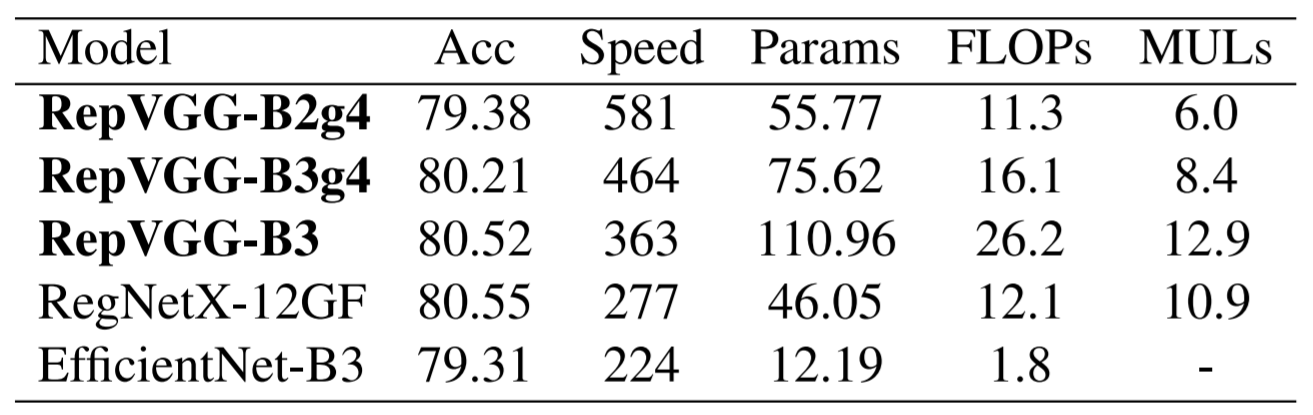
\includegraphics[width=0.8\linewidth]{images/results2.PNG}
	\end{center}
	\caption{RepVGG performance on ImageNet after being trained 200 epochs with Autoaugment, label smoothing and mixup.}
	\label{fig:results2}
\end{figure}

The fact that RepVGG as the first of its kind achieved an accuracy of over 80\% on ImageNet is also not to forget (see \autoref{fig:results2}).

\subsection{Ablation studies}

\begin{figure}[t]
	\begin{center}
		% \fbox{\rule{0pt}{2in}\rule{0.9\linewidth}{0pt}}
		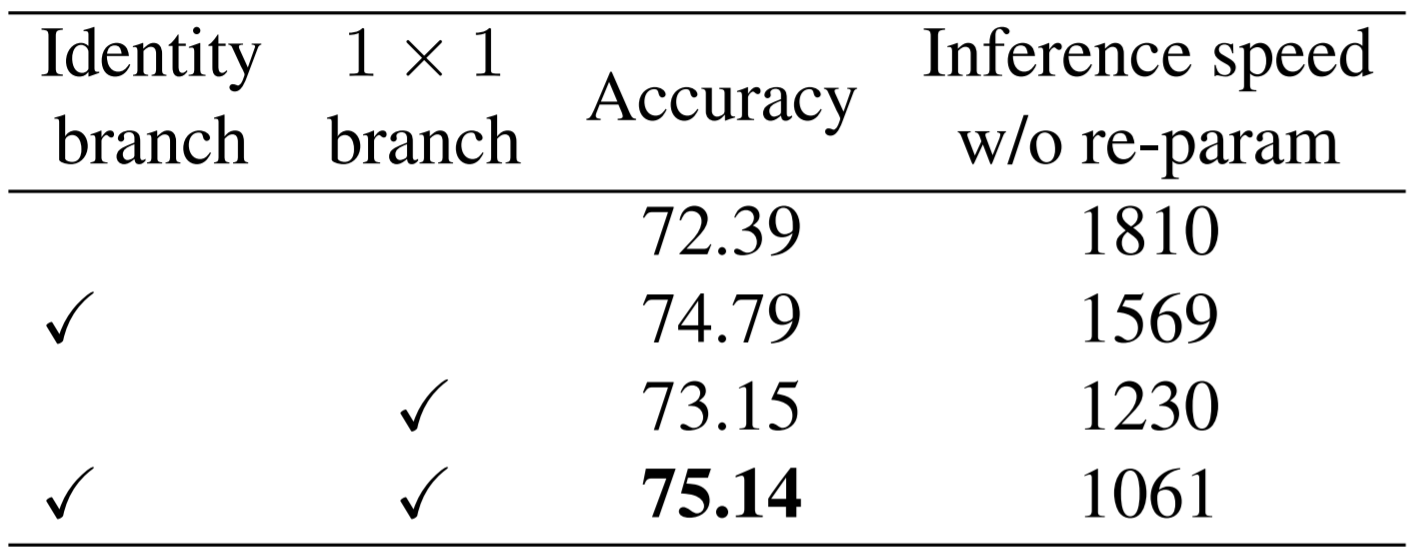
\includegraphics[width=0.8\linewidth]{images/ablation1.PNG}
	\end{center}
	\caption{Ablation studies with 120 epochs on RepVGG-B0}
	\label{fig:ablation1}
\end{figure}

In the ablation studies in \autoref{fig:ablation1} one recognizes the importance of the skip-connections and ensemble character of RepVGG after 120 epochs of training as the performance decreases when removing the identity and/or 1x1 convolutional branches. At the same time the speed increases when switching from a multi-branch model to a single-branch model. Note that the speed is this time measured before the structural re-parameterization. 

\begin{figure}[t]
	\begin{center}
		% \fbox{\rule{0pt}{2in}\rule{0.9\linewidth}{0pt}}
		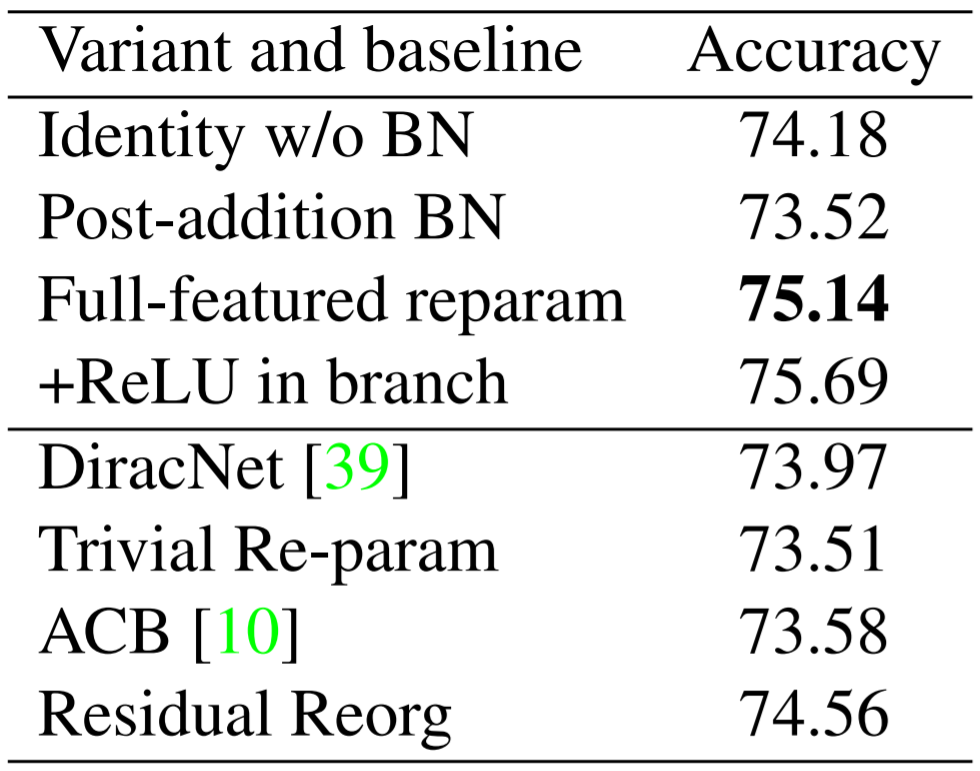
\includegraphics[width=0.8\linewidth]{images/ablation2.PNG}
	\end{center}
	\caption{Performance comparisons with architectural variants of RepVGG-B0}
	\label{fig:ablation2}
\end{figure}

The experiments shown in \autoref{fig:ablation2} are based on architectural changes of RepVGG-B0 after being trained for 120 epochs. With experiments using a DiracNet-like re-parameterization, a trivial re-parameterization (DiracNet re-parameterization with both scaling factors $a$ and $b$ set constant to one) and another structural re-parameterization method with asymmetric convolutional blocks, interesting experiments and comparisons to other methods of re-parameterization are given. One can therefore conclude, that re-parameterization with parameters only simulating a ResNet-like architecture during training like DiracNet does is inferior to a real structural re-parameterization method like RepVGG uses. Also the success of RepVGG cannot be traced back to simple over-parameterization of each block during training when comparing the accuracy of an initial RepVGG-B0 model to a similar model with plugged-in ACB blocks replacing the RepVGG blocks. Both models therefore use over-parameterization during training and afterwards structural re-parameterization to build the inferecne model, still the RepVGG model yields in higher accuracy. RepVGG is specifically designed to make plain VGG-like CNNs trainable and achieves its higher accuracy compared to a ACB-enriched architecture through its ResNet-like training-time architecture. 

For the last comparison made in the experiments, a real residual network having one 3x3 convolutional layer in the first stage and two, three and eight residual blocks in stage two, three and four was build (skip-connections just like ResNet-18/34). While having the same amount of 3x3 conv layers RepVGG still managed to outperform such an architecture (75.14 vs. 74.56), which is not surprising looking back at the first experiments made and keeping in mind that RepVGG can be seen as an ensemble of far more models. 
